\chapter{Numerical Simulations and Results \label{results}}
\section{Comparison with other numerical solutions to the Eady Frontogenesis Model}
\subsection{Evolution of Average Kinetic Energy}
The kinetic energy over the domain $\Gamma$ is defined by,
\begin{equation}
	E_{kin} = \int_\Gamma \ \frac{1}{2}v_g^2 \ dxdz
	\label{KE1}
\end{equation}
Given the geostrophic transformation \ref{geostrophictransformation} this can be expressed as,
\begin{equation}
E_{kin} = \int_\Gamma \ \frac{f^2}{2}(X-x)^2 \ dxdz
\label{KE2}
\end{equation}
The kinetic energy associated with a fluid particle is the similarly defined as the integrals \ref{KE1} and \ref{KE2} but over the Laguerre cell of the point and its associated weight given by the solution of the optimal transport problem.
\comments{sort out domain averaged, show that solutions converge}
\section{Error Analysis of the numerical Solution}
\comments{discuss enery as error measurment, log-log plots for euler and heun and way to reduce error}
\section{Computational Performance}
\chapter{Unsorted}
\section{Linear Stability Analysis}
Starting from the Eady Model \ref{EadyModel} restated below
\begin{equation}
\begin{aligned}
-fv_g + \frac{\partial \varphi}{\partial x} = 0,\\
\frac{Dv_g}{Dt} + fu -\frac{Cg}{\theta _0}\left(z-H/2\right) = 0,\\
\frac{D\theta'}{Dt} - Cv_g = 0,\\
\frac{\partial \varphi}{\partial z} - g\frac{\theta'}{\theta_0} = 0,\\
\nabla \cdot \bm{u} = 0.
\end{aligned}
\label{EadyModel2}
\end{equation} 
Linearise about a base state given by Hoskins \cite{Hoskins1975},
\begin{equation}
\begin{aligned}
\bar{\theta} &= \theta_0 \frac{N_0^2\theta_0 z}{g} - Cy \\
\bar{\varphi} &= \theta_0 + \frac{N_0^2 z^2}{2}\\
\bar{v}_g &= 0\\
\bar{U} &= \frac{Cg}{f\theta_0}\left(z - H/2\right)\\
\bar{W} &= 0 
\end{aligned}
\end{equation}
Introduce a perturbation and linearise about base state,\\
$u = \bar{U} + u'$, $w = w'$, $v_g =  v_g'$, $\varphi = \bar{\varphi} + \varphi'$, $\theta ' = \bar{\theta} + \theta ''$\\
Introducing the stream function,
\begin{equation}
u' = \frac{\partial \psi}{\partial z},\qquad w' = -\frac{\partial \psi}{\partial x} 
\end{equation}
Looking for normal modes solutions of the form,
\begin{equation*}
q' = \hat{q}(z)\exp^{i \left(kx - \omega t\right)}
\end{equation*}
Equations \ref{EadyModel2} become,
\begin{align}
-f\hat{v}_g + ik\hat{\varphi} = 0,\label{stab1}\\
-i\omega \hat{v}_g + ik\bar{U}\hat{v}_g + f\frac{\text{d}\hat{\psi}}{\text{d}z} = 0,\label{stab2}\\
-i \omega \hat{\theta} + i k \bar{U} \hat{\theta} - ik\frac{N_0^2\theta_0}{g} \hat{\psi} - C\hat{v}_g = 0,\label{stab3}\\
\frac{\text{d}\hat{\varphi}}{\text{d}z} - g\frac{\hat{\theta}}{\theta_0} = 0 \label{stab4},
\end{align}
First eliminating, $\varphi$, equations \ref{stab1} and \ref{stab4} give,
\begin{equation*}
-f\frac{\text{d}\hat{v}_g}{\text{d}z}+ik\frac{\text{d}\hat{\varphi}}{\text{d}z} = 0, \qquad \frac{\text{d}\hat{\varphi}}{\text{d}z} - g\frac{\hat{\theta}}{\theta_0} = 0
\end{equation*}
so that,
\begin{equation}
\hat{\theta} = \frac{f\theta_0}{ikg} \frac{\text{d}\hat{v}_g}{\text{d}z}
\label{thetahat}
\end{equation}
Rearranging equation \ref{stab3}
\begin{equation}
i\left( k \bar{U} - \omega \right) \hat{\theta} - ik\frac{N_0^2\theta_0}{g} \hat{\psi} - C\hat{v}_g = 0
\label{stab3.1}
\end{equation}
Eliminating $\hat{\theta}$ using \ref{thetahat}
\begin{equation*}
\frac{f\theta_0}{kg}\left( k \bar{U} - \omega \right)  \frac{\text{d}\hat{v}_g}{\text{d}z} - ik\frac{N_0^2\theta_0}{g} \hat{\psi} - C\hat{v}_g = 0
\end{equation*}
from equation \ref{stab2} we have
\begin{equation}
i\left( k \bar{U} - \omega \right) \hat{v}_g - f \frac{\text{d}\hat{\psi}}{\text{d}z} = 0
\label{stab2.1}
\end{equation}
differentiating this expression we find
\begin{equation*}
ik \frac{\text{d}\bar{U}}{\text{d}z} \hat{v}_g + i(k\bar{U}-\omega)\frac{\text{d}\hat{v}_g}{\text{d}z} + f\frac{\text{d}^2{\psi}}{\text{d}z^2} = 0 
\end{equation*}
Substituting this expression with \ref{stab2.1} into \ref{stab3.1}, noting that,
\begin{equation*}
(k\bar{U}-\omega)\frac{\text{d}\hat{v}_g}{\text{d}z} = if\frac{\text{d}^2{\psi}}{\text{d}z^2} + \frac{fk}{i(k\bar{U}-\omega)}\frac{\text{d}\bar{U}}{\text{d}z}\frac{\text{d}\hat{\psi}}{\text{d}z}
\end{equation*}
\begin{equation*}
\frac{f\theta_0}{kg}\left(if\frac{\text{d}^2{\psi}}{\text{d}z^2} + \frac{fk}{i(k\bar{U}-\omega)}\frac{\text{d}\bar{U}}{\text{d}z}\frac{\text{d}\hat{\psi}}{\text{d}z}\right) - \frac{ik N_0^2\theta_0\hat{\psi}}{g} + \frac{Cf}{i(k\bar{U}-\omega)}\frac{\text{d}\psi}{\text{d}z} =0
\end{equation*}
Rearranging gives,
\begin{equation*}
-\frac{f^2\theta_0}{kg}(k\bar{U}-\omega)\frac{\text{d}^2{\psi}}{\text{d}z^2}+\left(Cf+\frac{f^2\theta_0}{g}\frac{\text{d}\bar{U}}{\text{d}z}\right)\frac{\text{d}\hat{\psi}}{\text{d}z}+\frac{k N_0^2\theta_0}{g}(k\bar{U}-\omega)\hat{\psi}=0
\end{equation*}
\begin{equation*}
-f^2\theta_0(k\bar{U}-\omega)\frac{\text{d}^2{\psi}}{\text{d}z^2}+2Cfkg\frac{\text{d}\hat{\psi}}{\text{d}z}+k^2 N_0^2\theta_0(k\bar{U}-\omega)\hat{\psi}=0
\end{equation*}
We reformulate this as a matrix eigenvalue problem for $\omega$
\begin{equation}
-f^2\theta_0\bar{U}\frac{\text{d}^2{\psi}}{\text{d}z^2}+2Cfkg\frac{\text{d}\hat{\psi}}{\text{d}z}+k^2 N_0^2\theta_0\bar{U}\hat{\psi}=\omega \left(k^2N_0^2\theta_0\hat{\psi}-f^2\theta_0 \frac{\text{d}^2{\psi}}{\text{d}z^2}\right)
\label{stabanalysis}
\end{equation}
Introducing a second order finite difference scheme for $\psi$
\begin{equation*}
\begin{aligned}
\frac{\text{d}^2{\hat{\psi}}}{\text{d}z^2} = \frac{\psi_{i-1} - 2\psi_i + \psi_{i+1}}{h^2}\\
\frac{\text{d}\hat{\psi}}{\text{d}z} = \frac{\psi_{i-1} - \psi_{i+1}}{2h}
\end{aligned}
\end{equation*}
Equation \ref{stabanalysis} becomes
\begin{equation}
\begin{aligned}
-f^2\theta_0\bar{U}_i\left(\frac{\psi_{i-1} - 2\psi_i + \psi_{i+1}}{h^2}\right)+2Cfkg\left(\frac{\psi_{i-1} -f \psi_{i+1}}{2h}\right)+k^3 N_0^2\theta_0\bar{U}_i\psi_i= \\
\omega\left(k^2N_0^2\theta_0\psi_i-f^2\theta_0\left(\frac{\psi_{i-1} - 2\psi_i + \psi_{i+1}}{h^2}\right)\right)
\end{aligned}
\end{equation}
Discretising the interval $[0,H]$ into $N$ points with step size $h$ we can recast this as an eigenvalue problem,
\begin{equation*}
A\bm{\psi} = \omega B\bm{\psi}
\end{equation*}
to find eigenvalues $\omega$ with corresponding eigenvectors $\bm{\psi} = \left(\psi_1, ... , \psi_{N-2}\right)$. Since the boundary condition gives $\psi = 0$ on $z = 0, H$, $\psi_0 = \psi_N = 0$ so these are omitted from the $\hat{\phi}$ vector but considered in the finite difference schemes for $\psi_1$ and $\psi_{N-1}$
The coefficients matrix $A$ are given by
\begin{equation}
\begin{aligned}
\psi_{i-1}:& \quad -\frac{-f^2\theta_0k\bar{U}_i}{h^2} - \frac{Cfkg}{h}\\
\psi_i:& \quad \frac{2f^2\theta_0k\bar{U}_i}{h^2} + k^3N_0^2\theta_0\bar{U}_i\\
\psi_{i+1}:& \quad \frac{-f^2\theta_0k\bar{U}_i}{h^2} + \frac{Cfkg}{h}\\
\end{aligned}
\end{equation}
$i: 1 \rightarrow N-2$ with $\psi_0 = \psi_{N}$. The coefficients of matrix $B$ are given by,
\begin{equation*}
\begin{aligned}
\psi_{i-1}:& \quad -\frac{f^2\theta_0}{h^2}\\
\psi_i:& \quad k^2N_0^2\theta_0 + \frac{2f^2\theta_0}{h^2}\\
\psi_{i+1}:& \quad -\frac{f^2\theta_0}{h^2}\\
\end{aligned}
\end{equation*}
\begin{figure}[h]
	\centering
	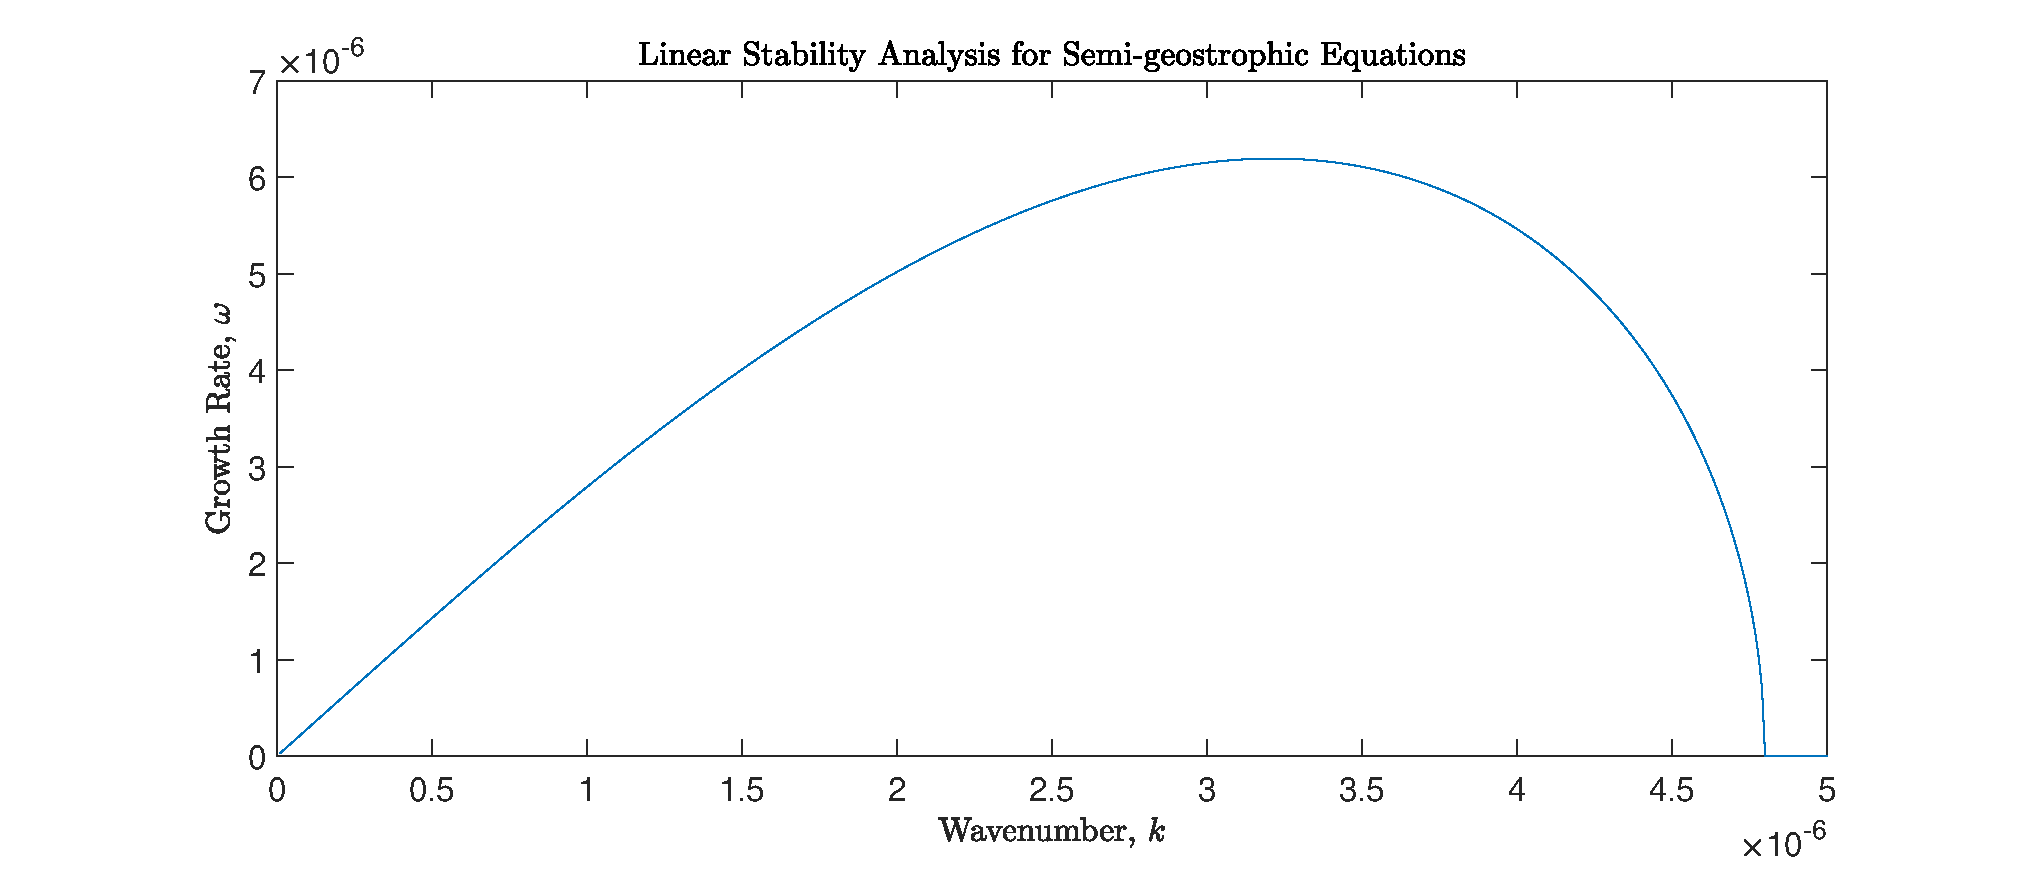
\includegraphics[width=\linewidth]{project/Linear_stability_analysis}
	\caption[Linear stability analysis results for the semi-geostrophic equations]{Plot showing growth rate, $\omega$ against wavenumber $k$ for the Eady model of the semi-geostrophic equations}
	\label{fig:linearstabilityanalysis}
\end{figure}
\section{Calculation of Moments}
For the implementation of the numerical algorithm for frontogenesis and subsequent analysis of its suitability, the moments of \comments{word choice} the cells are required. Consider a point in geostrophic space $\bm{Y} = \left(X,Z\right)$ in the fundamental domain and corresponding weight $\psi$ for which the Laguerre cell is $A = \mathrm{Lag}_{\bm{Y}}(\psi)$
\begin{description}
	\item [$\bm{O^{th}}$ Moment] 
	\begin{equation}
		M_0 = \int_A dxdz
	\end{equation}
	\item[$\bm{1^{st}}$ Moment]
	\begin{equation}
	M_{1x} = \int_A x dxdz, \qquad M_{1z} = \int_A z dxdz
	\end{equation}
	\item[$\bm{2^{nd}}$ Moment]
	\begin{equation}
	M_{2x} = \int_A x^2 dxdz, \qquad M_{2z} = \int_A z^2 dxdz, \qquad M_{2xz} = \int_A xz dxdz
	\end{equation}	
\end{description}

\subsection{Considerations for Periodic Boundary Conditions}
In implementing the moment calculations the periodicity of the domain needs to be carefully considered. For example, consider a point in geostrophic space $\left(X, Z\right)$ in the fundamental domain and corresponding weight $\psi$ it is possible that if $X$ lies close to one of the limit points of the interval $[-L,L]$, that the centroid of the Laguerre cell associated with this point is exterior to the fundamental domain.
\section{Ideas for extension}
